\chapter{Class Diagrams}

\section{Optimisation library Class Diagram}
\label{sec:appendix1}
\begin{landscape}
  \begin{figure}[h]
    \begin{center}
      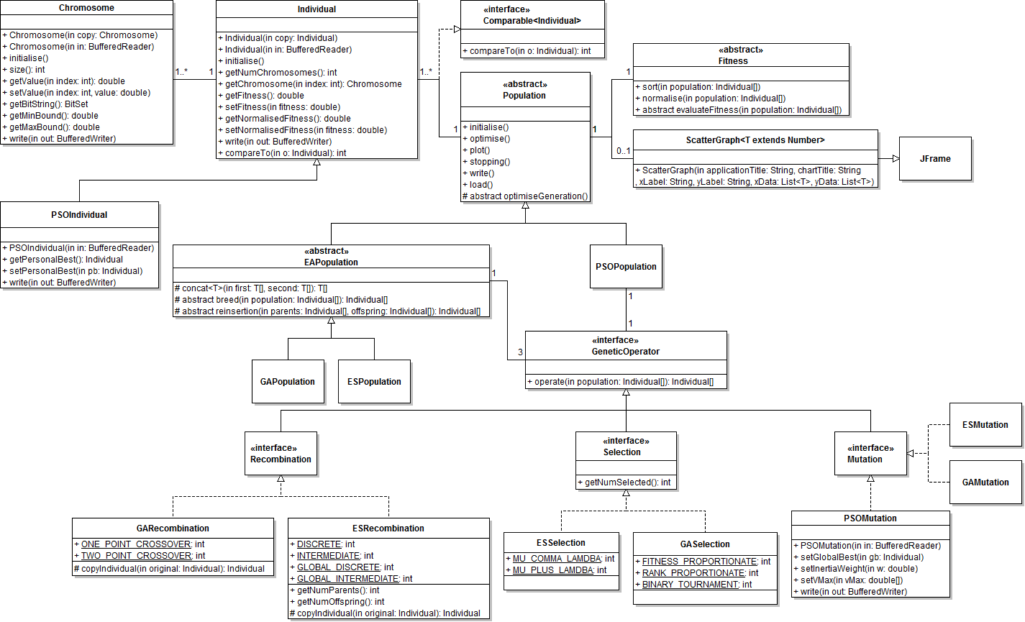
\includegraphics{Figures/generic_class_diagram}
    \end{center}
    \caption{Class diagram for the optimisation library}
    \label{fig:phase1}
  \end{figure}
\end{landscape}

\section{The Arena Class Diagram}
\label{sec:appendix2}
\begin{landscape}
  \begin{figure}[h]
    \begin{center}
      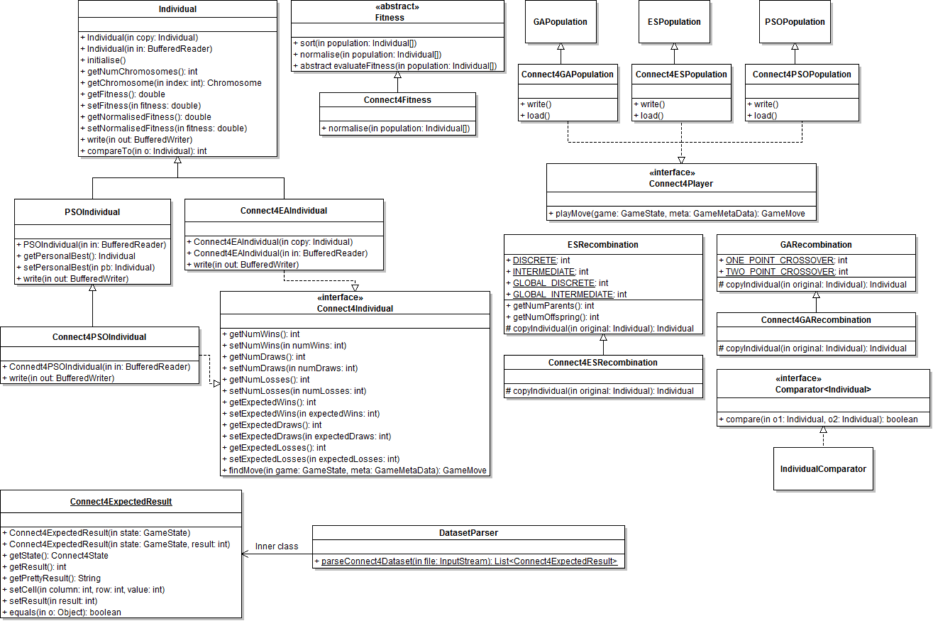
\includegraphics{Figures/connect_4_class_diagram}
    \end{center}
    \caption{Class diagram showing the additional Arena classes}
    \label{fig:phase2}
  \end{figure}
\end{landscape}

\chapter{Phase One Test Results}

\begin{landscape}
\section{Genetic Algorithm}
\subsection{Binary Tournament Selection With Two-point Crossover}
\label{sec:appendix3}
  \begin{figure}[h]
    \begin{center}
      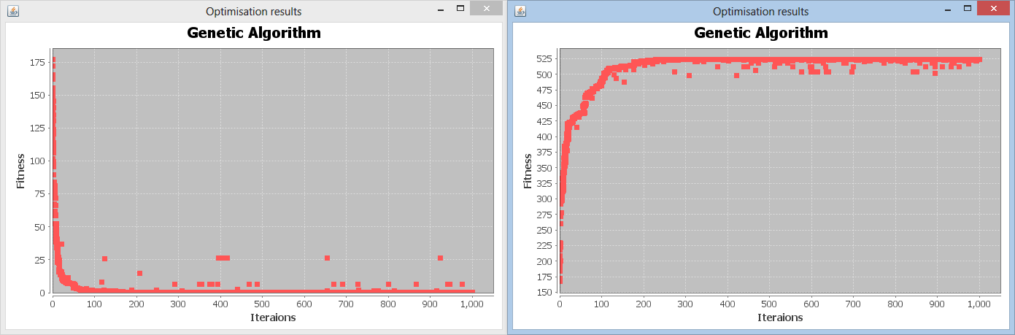
\includegraphics{Figures/ga_bt_2p}
    \end{center}
    \caption{Optimisation results of a genetic algorithm using binary tournament selection and two-point crossover}
    \label{fig:phase1}
  \end{figure}
\end{landscape}

\begin{landscape}
\subsection{Binary Tournament Selection With One-point Crossover}
\label{sec:appendix4}
  \begin{figure}[h]
    \begin{center}
      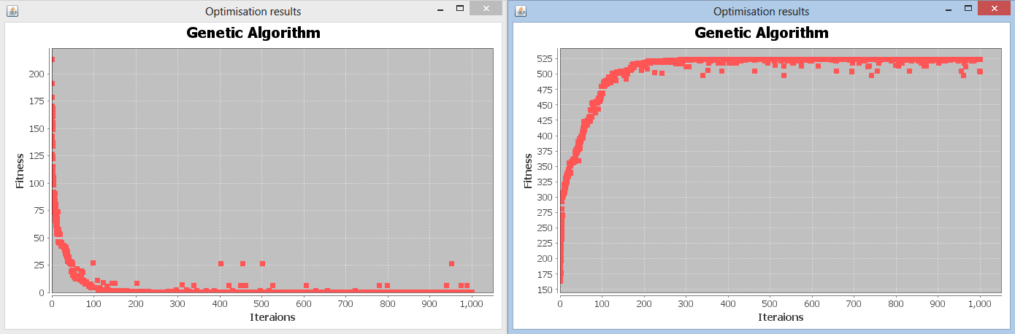
\includegraphics{Figures/ga_bt_1p}
    \end{center}
    \caption{Optimisation results of a genetic algorithm using binary tournament selection and one-point crossover}
    \label{fig:phase1}
  \end{figure}
\end{landscape}

\begin{landscape}
\subsection{Rank Selection With Two-point Crossover}
\label{sec:appendix5}
  \begin{figure}[h]
    \begin{center}
      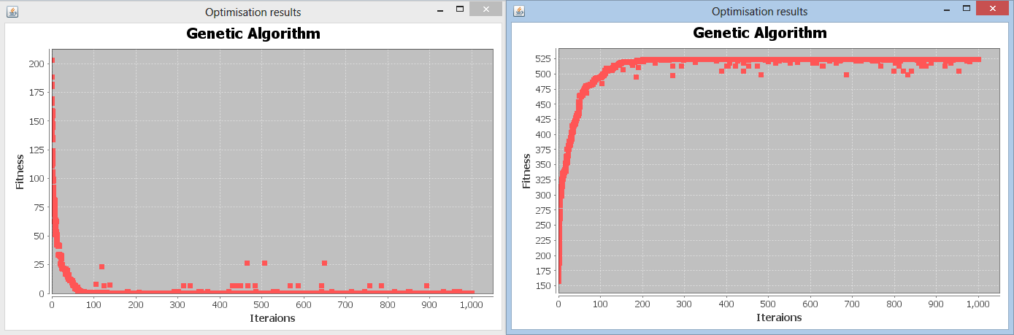
\includegraphics{Figures/ga_rp_2p}
    \end{center}
    \caption{Optimisation results of a genetic algorithm using rank selection and two-point crossover}
    \label{fig:phase1}
  \end{figure}
\end{landscape}

\begin{landscape}
\subsection{Rank Selection With One-point Crossover}
\label{sec:appendix6}
  \begin{figure}[h]
    \begin{center}
      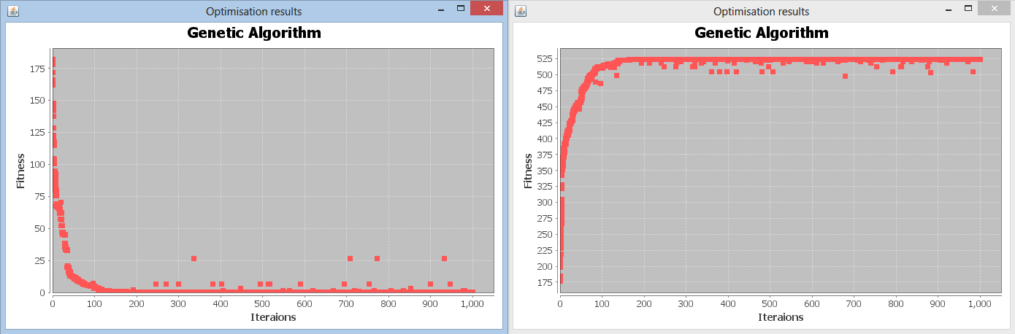
\includegraphics{Figures/ga_rp_1p}
    \end{center}
    \caption{Optimisation results of a genetic algorithm using rank selection and one-point crossover}
    \label{fig:phase1}
  \end{figure}
\end{landscape}

\begin{landscape}
\subsection{Proportional Selection With Two-point Crossover}
\label{sec:appendix7}
  \begin{figure}[h]
    \begin{center}
      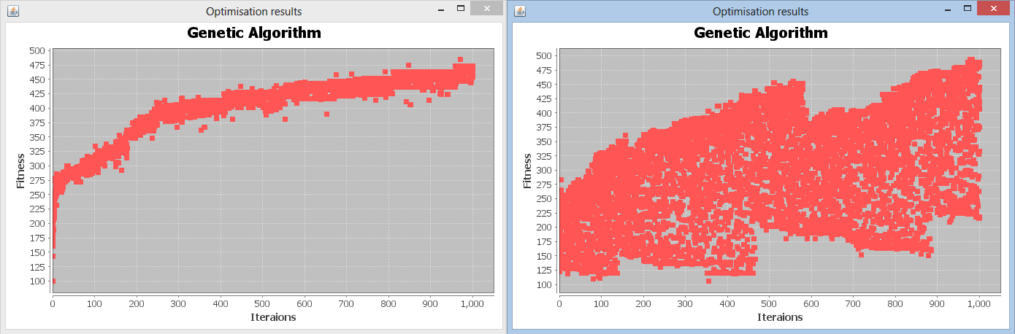
\includegraphics{Figures/ga_fp_2p}
    \end{center}
    \caption{Optimisation results of a genetic algorithm using proportional selection and two-point crossover}
    \label{fig:phase1}
  \end{figure}
\end{landscape}

\begin{landscape}
\subsection{Proportional Selection With One-point Crossover}
\label{sec:appendix8}
  \begin{figure}[h]
    \begin{center}
      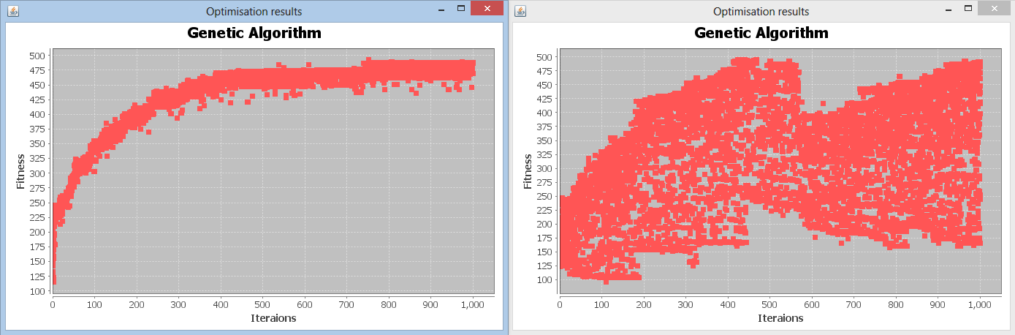
\includegraphics{Figures/ga_fp_1p}
    \end{center}
    \caption{Optimisation results of a genetic algorithm using proportional selection and one-point crossover}
    \label{fig:phase1}
  \end{figure}
\end{landscape}

\begin{landscape}
\subsection{Proportional Selection With Adjusted Numbers of Parents}
\label{sec:appendix9}
  \begin{figure}[h]
    \begin{center}
      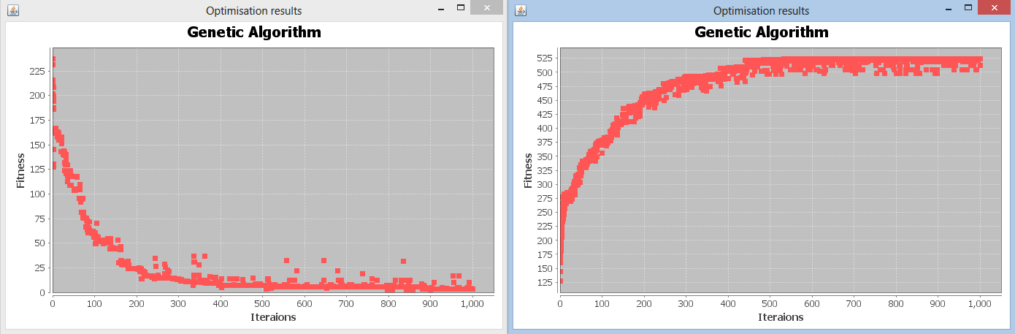
\includegraphics{Figures/ga_fp_2p_parents}
    \end{center}
    \caption{Optimisation results of a genetic algorithm using proportional selection and two-point crossover. The number of parents has been adjusted to give better results.}
    \label{fig:phase1}
  \end{figure}
\end{landscape}

\begin{landscape}
\subsection{Binary Tournament Selection With Two-point Crossover in Shark}
\label{sec:appendix10}
  \begin{figure}[h]
    \begin{center}
      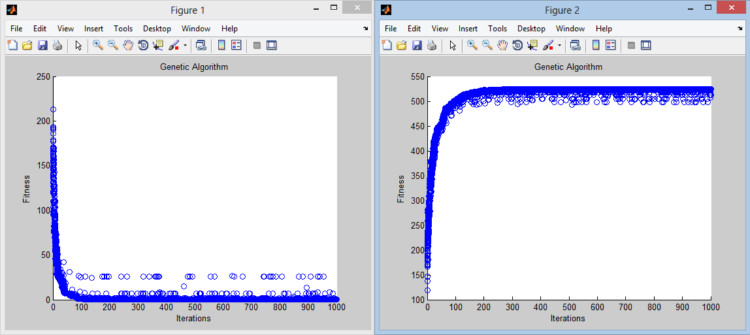
\includegraphics{Figures/sharkga}
    \end{center}
    \caption{Optimisation results of a genetic algorithm using binary tournament selection and two-point crossover implemented in Shark}
    \label{fig:phase1}
  \end{figure}
\end{landscape}

\begin{landscape}
\section{Evolution Strategies}
\subsection{$(\mu,\lambda)$ Selection With Discrete Recombination}
\label{sec:appendix11}
  \begin{figure}[h]
    \begin{center}
      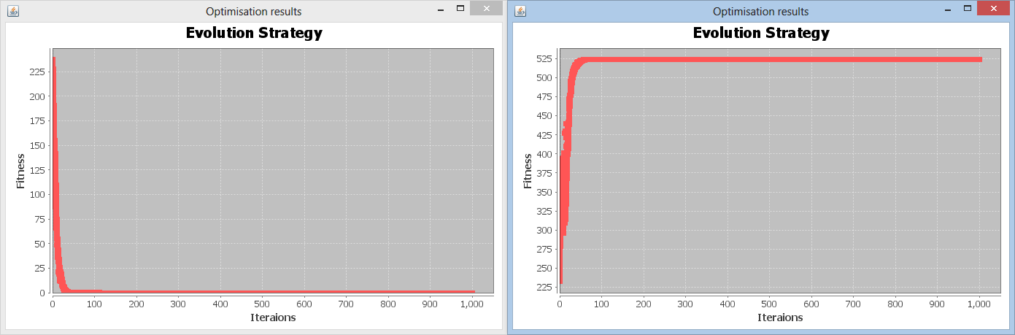
\includegraphics{Figures/es_comma_d}
    \end{center}
    \caption{Optimisation results of evolution strategies using $(\mu,\lambda)$ selection and discrete recombination}
    \label{fig:phase1}
  \end{figure}
\end{landscape}

\begin{landscape}
\subsection{$(\mu,\lambda)$ Selection With Intermediate Recombination}
\label{sec:appendix12}
  \begin{figure}[h]
    \begin{center}
      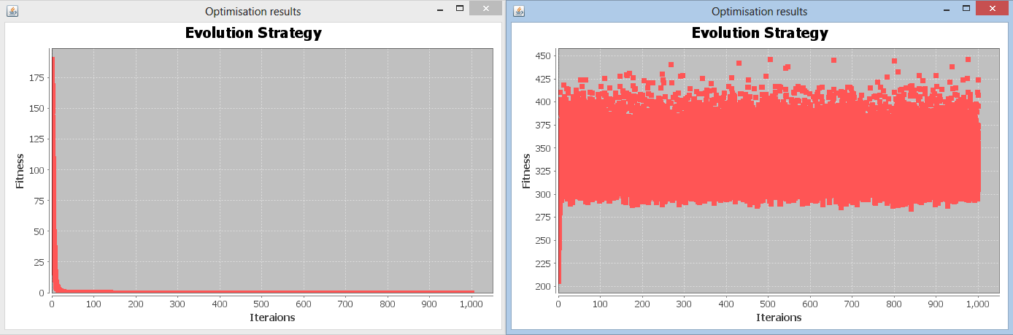
\includegraphics{Figures/es_comma_i}
    \end{center}
    \caption{Optimisation results of evolution strategies using $(\mu,\lambda)$ selection and intermediate recombination}
    \label{fig:phase1}
  \end{figure}
\end{landscape}

\begin{landscape}
\subsection{$(\mu,\lambda)$ Selection With Global Discrete Recombination}
\label{sec:appendix13}
  \begin{figure}[h]
    \begin{center}
      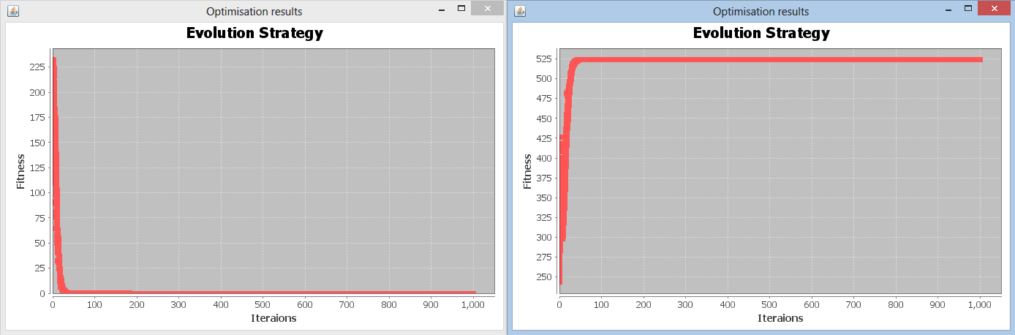
\includegraphics{Figures/es_comma_gd}
    \end{center}
    \caption{Optimisation results of evolution strategies using $(\mu,\lambda)$ selection and global discrete recombination}
    \label{fig:phase1}
  \end{figure}
\end{landscape}

\begin{landscape}
\subsection{$(\mu,\lambda)$ Selection With Global Intermediate Recombination}
\label{sec:appendix14}
  \begin{figure}[h]
    \begin{center}
      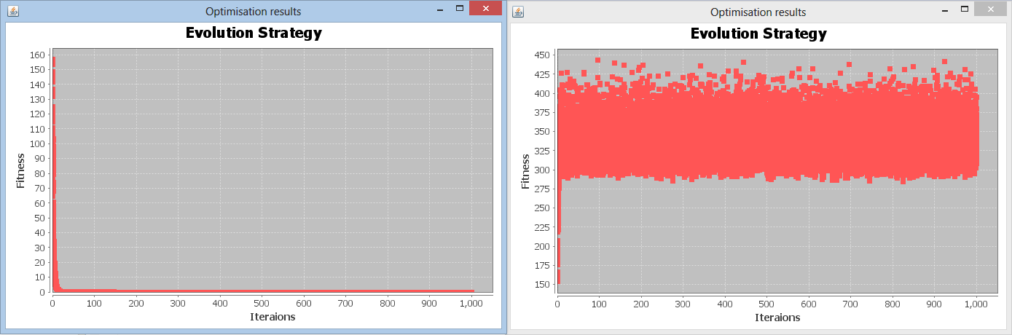
\includegraphics{Figures/es_comma_gi}
    \end{center}
    \caption{Optimisation results of evolution strategies using $(\mu,\lambda)$ selection and global intermediate recombination}
    \label{fig:phase1}
  \end{figure}
\end{landscape}

\begin{landscape}
\subsection{$(\mu+\lambda)$ Selection With Discrete Recombination}
\label{sec:appendix15}
  \begin{figure}[h]
    \begin{center}
      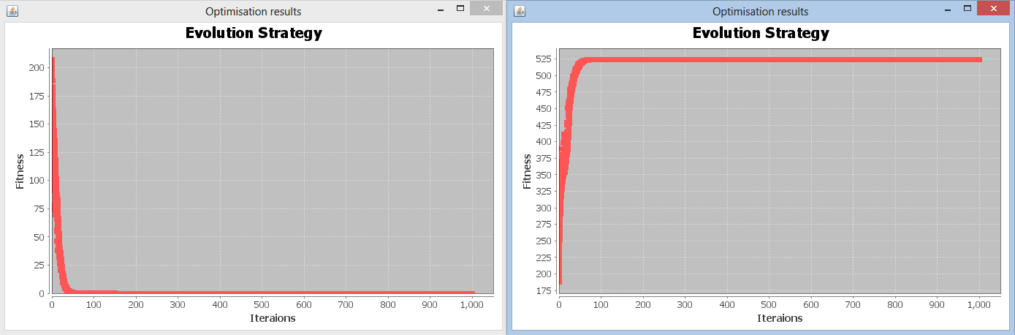
\includegraphics{Figures/es_plus_d}
    \end{center}
    \caption{Optimisation results of evolution strategies using $(\mu+\lambda)$ selection and discrete recombination}
    \label{fig:phase1}
  \end{figure}
\end{landscape}

\begin{landscape}
\subsection{$(\mu+\lambda)$ Selection With Intermediate Recombination}
\label{sec:appendix16}
  \begin{figure}[h]
    \begin{center}
      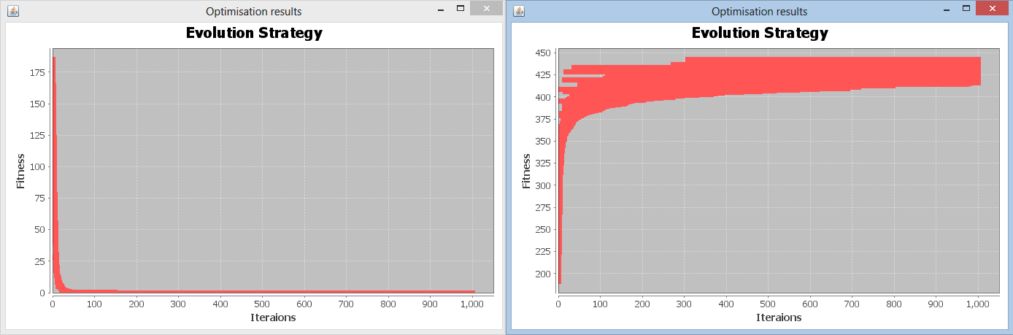
\includegraphics{Figures/es_plus_i}
    \end{center}
    \caption{Optimisation results of evolution strategies using $(\mu+\lambda)$ selection and intermediate recombination}
    \label{fig:phase1}
  \end{figure}
\end{landscape}

\begin{landscape}
\subsection{$(\mu+\lambda)$ Selection With Global Discrete Recombination}
\label{sec:appendix17}
  \begin{figure}[h]
    \begin{center}
      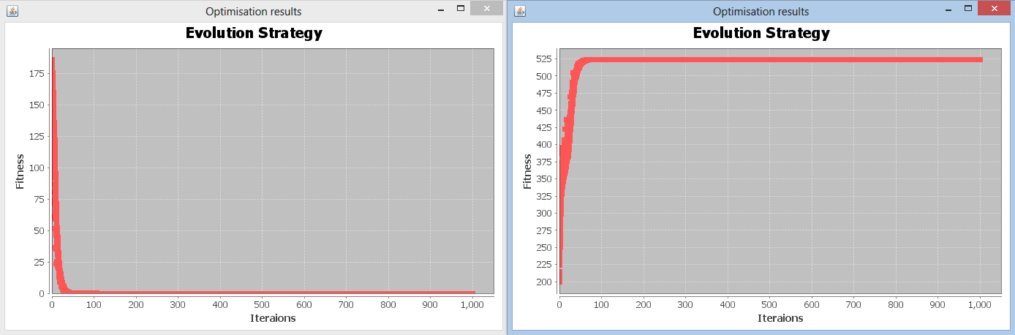
\includegraphics{Figures/es_plus_gd}
    \end{center}
    \caption{Optimisation results of evolution strategies using $(\mu+\lambda)$ selection and global discrete recombination}
    \label{fig:phase1}
  \end{figure}
\end{landscape}

\begin{landscape}
\subsection{$(\mu+\lambda)$ Selection With Global Intermediate Recombination}
\label{sec:appendix18}
  \begin{figure}[h]
    \begin{center}
      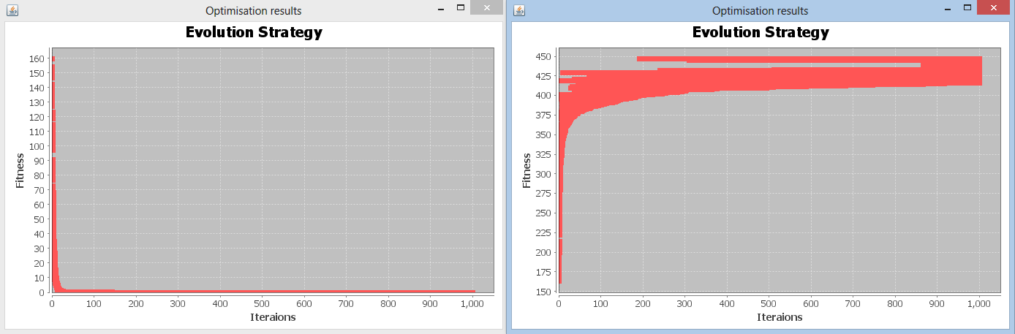
\includegraphics{Figures/es_plus_gi}
    \end{center}
    \caption{Optimisation results of evolution strategies using $(\mu+\lambda)$ selection and global intermediate recombination}
    \label{fig:phase1}
  \end{figure}
\end{landscape}

\begin{landscape}
\subsection{$(\mu+\lambda)$ Selection With Discrete Recombination in Shark}
\label{sec:appendix19}
  \begin{figure}[h]
    \begin{center}
      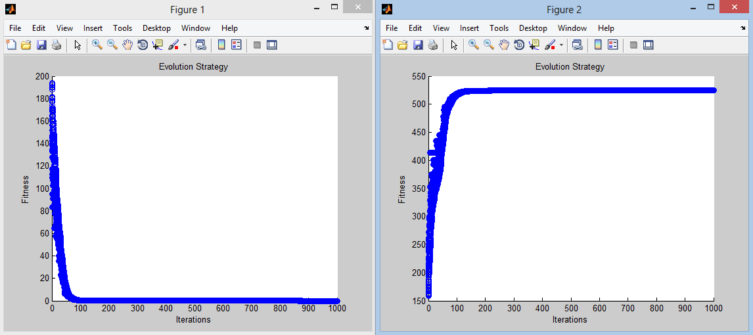
\includegraphics{Figures/sharkes}
    \end{center}
    \caption{Optimisation results of evolution strategies using $(\mu+\lambda)$ selection and discrete recombination implemented in Shark}
    \label{fig:phase1}
  \end{figure}
\end{landscape}

\begin{landscape}
\section{Particle Swarm Optimisation}
\subsection{Optimisation Results}
\label{sec:appendix20}
  \begin{figure}[h]
    \begin{center}
      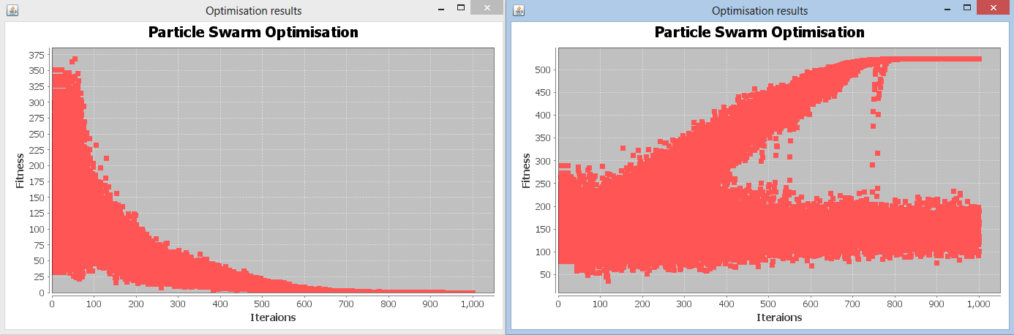
\includegraphics{Figures/pso}
    \end{center}
    \caption{Optimisation results of particle swarm optimisation}
    \label{fig:phase1}
  \end{figure}
\end{landscape}

\begin{landscape}
\subsection{Optimisation Results in Shark}
\label{sec:appendix21}
  \begin{figure}[h]
    \begin{center}
      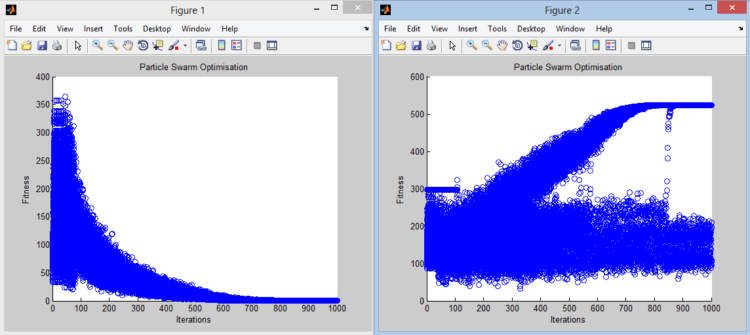
\includegraphics{Figures/sharkpso}
    \end{center}
    \caption{Optimisation results of particle swarm optimisation implemented in Shark}
    \label{fig:phase1}
  \end{figure}
\end{landscape}